
\documentclass[../../tex_main/NEMO_manual]{subfiles}

\begin{document}

% ================================================================
% Chapter 2 � Domain
% ================================================================

\chapter{Time, space and thickness space domain}
\label{chap:DOM}
\minitoc

\newpage
$\ $\newline    % force a new line
Excel
\section{Time domain}

Time stepping. Dynamics then thermodynamics. nn\_fsbc. EVP subcycles. 

\section{Spatial domain}

Not much to say about domain. Handled by NEMO. C-grid. Scale factors.

Vertical layers (nlay\_i, nlay\_s)

\section{Thickness category boundaries}

[ jpl, nn\_virtual\_itd ]

2 formulations to describe

[ ln\_cat\_hfn (function), rn\_himean ]

ln\_cat\_usr (user defined), rn\_catbnd, rn\_himin
Categories: boundary definitions. 
See doc 2.0, there are commented bits of text in the tex file.

Recall recommendations from Francois's, Antoine et al's paper.

%%--------------------------------------------------------------------------------------------------------------------
%%
%% FIGx : Ice categories
%%
%%
%\begin{figure}[ht]
%\begin{center}
%\vspace{0cm}
%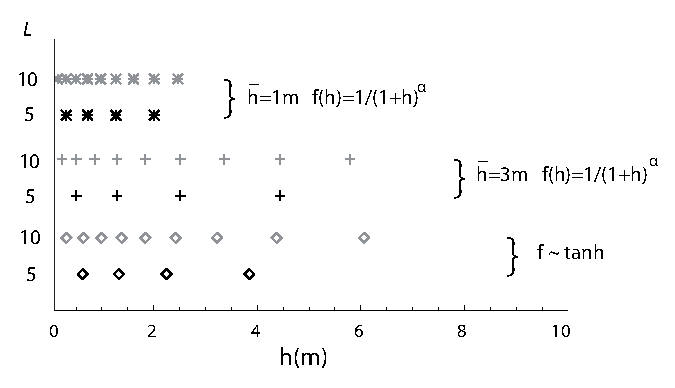
\includegraphics[height=6cm,angle=-00]{./Figures/ice_cats_new.eps}
%\caption{\footnotesize{Boundaries of the model ice thickness categories (m) for varying number of categories, prescribed mean thickness ($\overline h$ and formulation}}\label{ice_cats}
%\end{center}
%\end{figure}
%%
%%--------------------------------------------------------------------------------------------------------------------
%
%The thickness distribution function $g(h)$ is numerically discretized into several ice thickness categories. The numerical formulation of the thickness categories follows Bitz et al. (2001) and Lipscomb (2001). A fixed number $L$ of thickness categories with a typical value of $L=5$ is imposed. For some variables, sea ice in each category is further divided into N vertical layers of ice and one layer of snow. In the remainder of the text, the $l=1, ..., L$ index runs for ice thickness categories and $k=1, ..., N$ for the vertical ice layers. 
%
%Each thickness category has a mean thickness $h^i_l$ ranging over $[H^*_{l-1}$, $H^*_{l}$]. $H^*_{0}=0$, while the other boundaries are typically chosen with greater resolution for thin ice.
%
%There are two options for discretization in $h$-space, illustrated in Fig. \ref{ice_cats}. 
%
%\textbf{1.} The tanh hyperbolic formulation from CICE.
%\begin{linenomath}
%\begin{align}
%H^*_l &= H^*_{l-1} + \frac{3}{L} + \frac{30}{L} \biggr [ 1 + tanh \biggr ( \frac{3l - 3 - 3L}{L} \biggr ) \biggr] \quad (l=1, ..., L-1).
%\end{align}
%\label{eq_301}
%\end{linenomath}
%The upper boundary $H^*_L$ is set to a very high value (99.).
%
%\textbf{2.} An adjustable home-made $1/h^\alpha$ formulation.
%
%To construct the discretization in $h$-space, we first prescribe $H^*_0$ and $H^*_L=H_{max}$. We then introduce a fitting function $f$, defined over $[0,\infty]$, stricly positive and decreasing. We impose that the $H^*_l$'s must be such that  their images in the $f$-space ($f_l = f(H^*_l)$) are equally spaced. In mathematical terms:
%\begin{eqnarray}
%f_l & = & f_0 - l \Delta f  \qquad (l = 2, ..., L-1),
%\label{eq_fl}
%\end{eqnarray}
%where $\Delta f = \frac{f_0 - f_L}{L}$.
%
%Let us now construct a discretization in $h$-space. We use the function $f(h)=1/(h+1)^\alpha$, where $\alpha$ is strictly positive;  and impose that $H^*_{max}=3\overline h$, where $\overline h$ is the mean thickness in the domain $\overline h$. Replacing in $\ref{eq_fl}$, we get:
%\begin{eqnarray} 
%H^*_l = \left ( \frac{ L ( H^*_L + 1 ) ^\alpha}{(L-l)( H^*_L + 1 ) ^\alpha + l} \right ) ^{1/\alpha} - 1
%\end{eqnarray}
%\label{intro}
%There are two parameters to tune: $\overline h$ and $\alpha$ (typically 0.05, used for Fig. \ref{ice_cats}).
%
%Each ice category has its own set of global state variables

\end{document}